\documentclass[xcolor=dvipsnames,hyperref={pdfpagelabels=false}]{beamer}

\usetheme{Boadilla}

\newcommand{\bi}{\begin{itemize}}
\newcommand{\ei}{\end{itemize}}
\newcommand{\be}{\begin{enumerate}}
\newcommand{\ee}{\end{enumerate}}
\newcommand{\bc}{\begin{center}}
\newcommand{\ec}{\end{center}}
\newcommand{\bd}{\begin{description}}
\newcommand{\ed}{\end{description}}
\newcommand{\I}{\item}
\newcommand{\f}{\frame}
\newcommand{\ft}{\frametitle}

\title{Offline Software Overview}
\subtitle{GlueX Collaboration Meeting}
\author[Mark Ito]{Mark M.\ Ito}
\date{February 21, 2014}
\institute[JLab]{Jefferson Lab}

\begin{document}

\f{\titlepage}

\f{\ft{Other Related Talks}
\bi
\I Software Review (Curtis, Opening Session)
\I Online Data Challenge (David, Online Session)
\I Tracking Improvements (Simon, this session)
\I Offline Data Challenge (Curtis, this session)
\ei
}

\f{

\bi
\I We have a data management plan
  \bi
  \I document hierarchy developed Lab-wide
  \I meeting with Library School folks from CMU
    \bi
    \I same problem as us: funding agencies want to to see this
    \ei
  \ei
\I Data Flow Tools
  \bi
  \I at JLab, a requirements document drafted by a committee
  \I implementation slowed by re-organization
  \I will not be ready for this data challenge
  \ei
\ei
}

\f{
$$
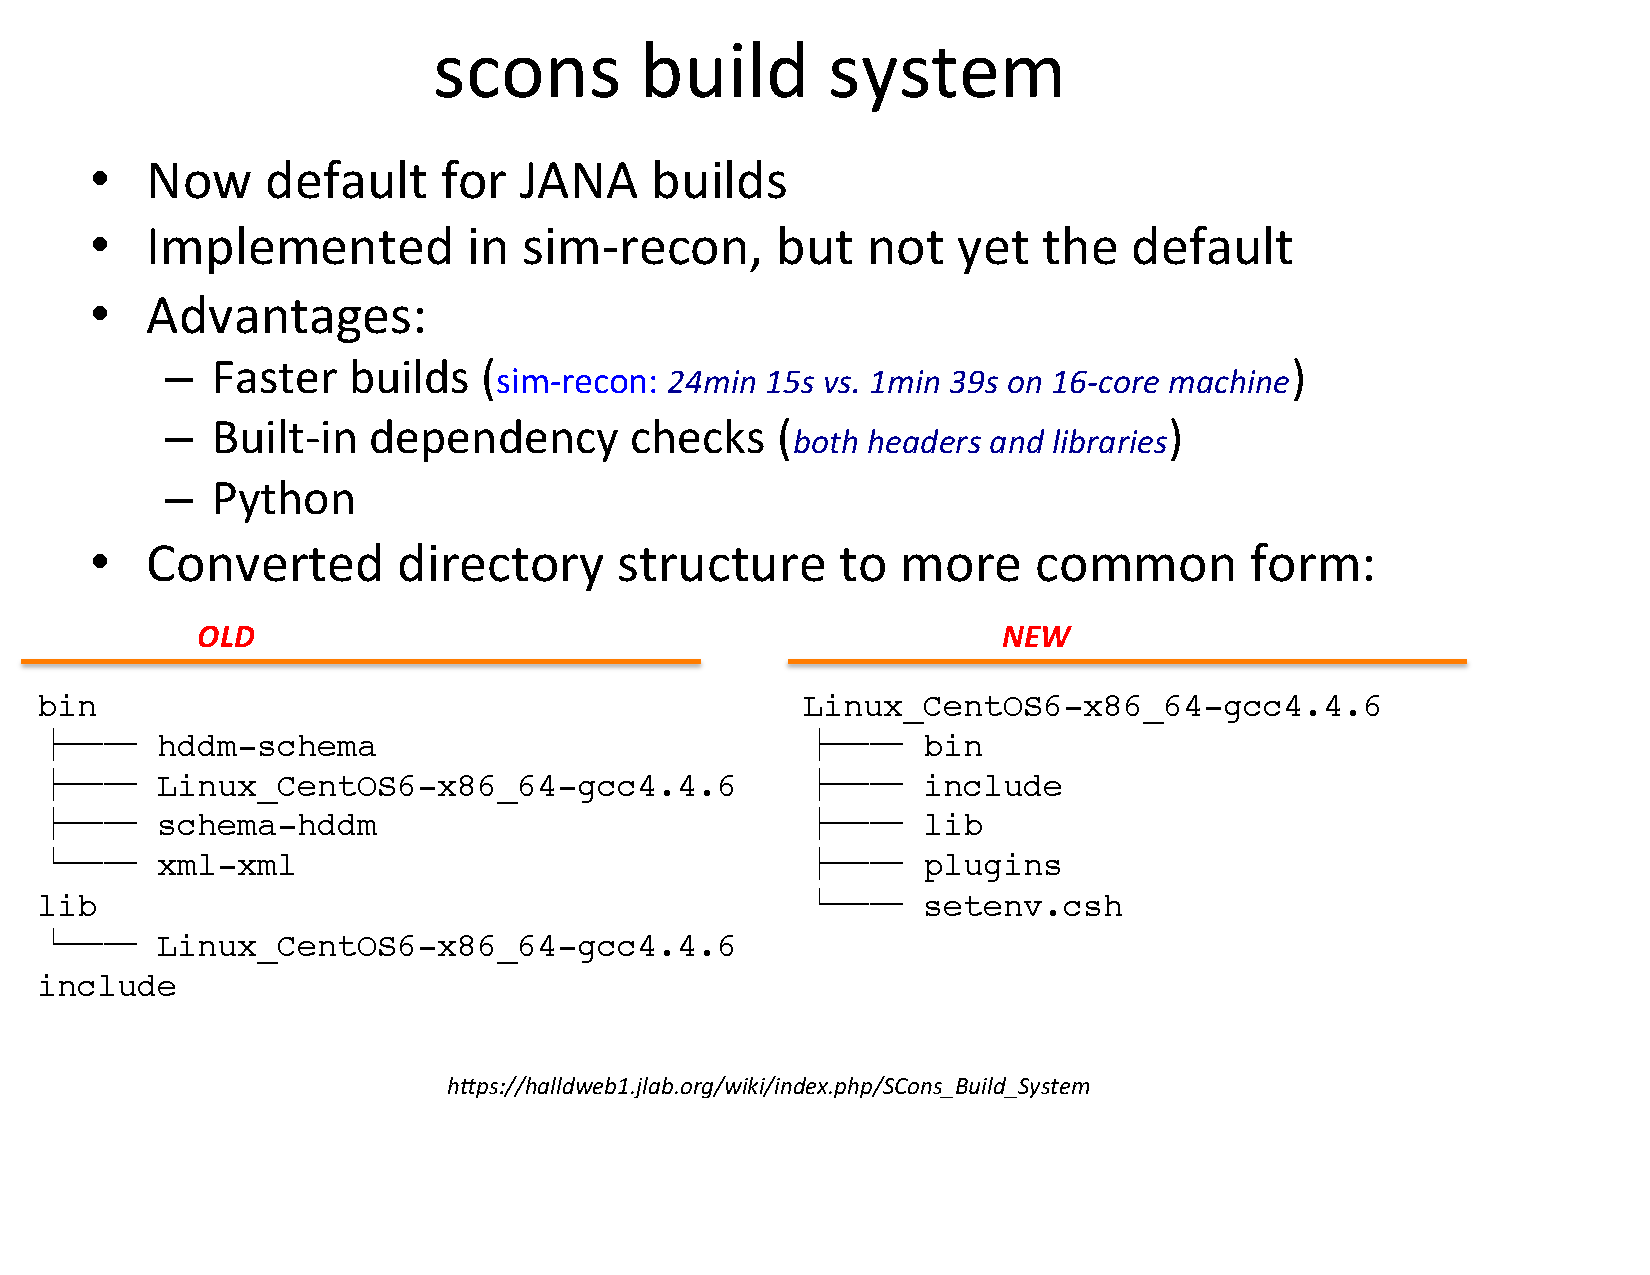
\includegraphics[width=\textwidth]{scons.pdf}
$$
}

\f{$$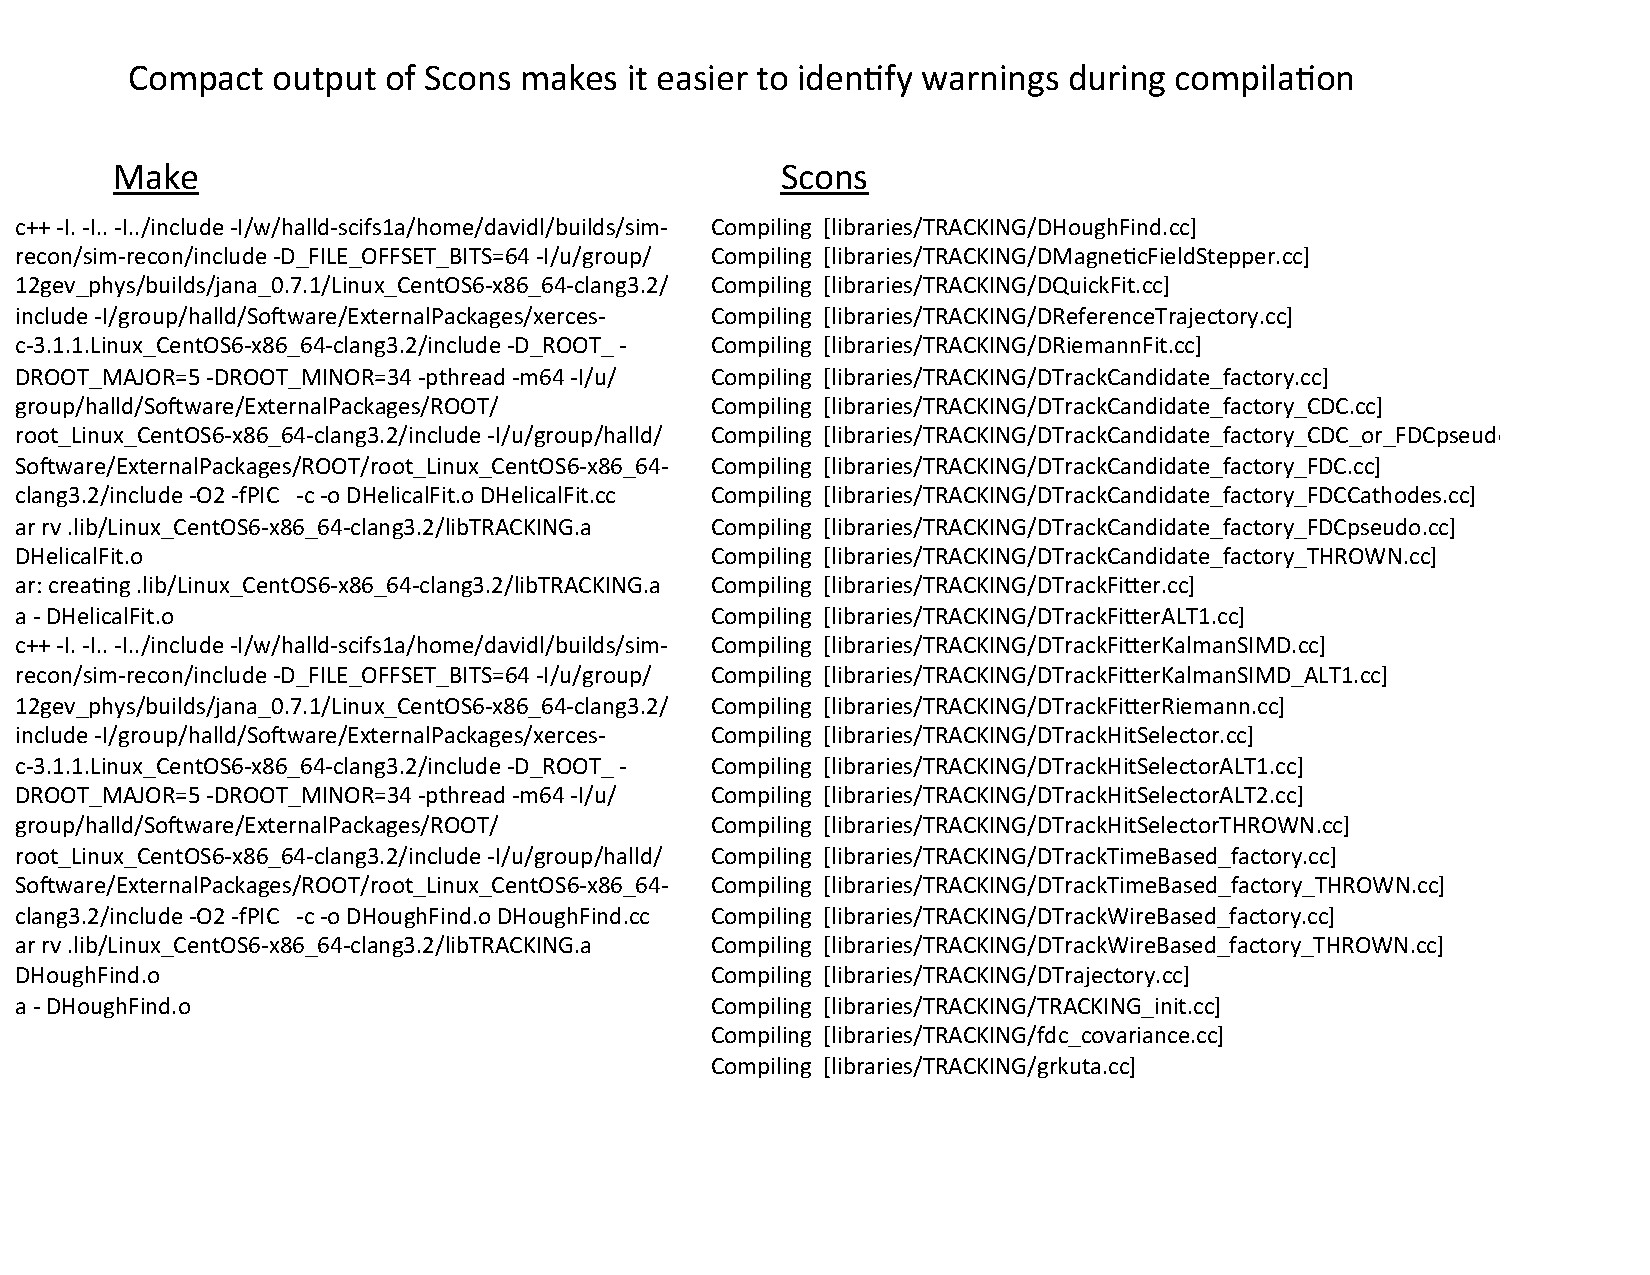
\includegraphics[width=\textwidth]{build_output.pdf}$$}
  
\f{
\bi
\I Monte Carlo Genealogy
  \bi
  \I scheme that allows family tree to cross over from bggen to hdgeant
  \ei
\I REST Format and Track Swimming
  \bi
  \I before: no information on cluster matching to tracks saved
  \I now: matching information kept in REST format
  \ei
\I CCDB, version 0.09
  \bi
  \I gateway for access to resources
  \I closes idle MySQL connections
  \I general improvements: help pages, better unit testing, documentation updates, web-site tweaks
  \I authentication implemented
  \I plan for Halls A and C to adopt use
  \I SQLite versions of CCDB generated automatically, daily
  \ei
\ei
}

\f{
\bi
\I Splitting up the packages
  \bi
  \I major categories: simulation, reconstruction, analysis
  \I other stand-alone candidates: AmpTools, HDDM, ``utilities''
  \I addresses some issues with old data
  \I still in planning stage
  \ei
\I Tagged File System for Event Data
  \bi
  \I Event file distribution
  \I tags: identify relevant files
  \I filters: select out events of interest
  \ei
\I EventStore being explored
  \bi
  \I system for tagging individual events
  \I used at CLEO
  \ei
\I Reverse Magnetic Field Fix
  \bi
  \I some non-generalities in code exposed
  \I allows for use of new magnetic field with the proper sign
  \ei
\I Time-of-Flight Geometry Changes
  \bi
  \I added half-width counters
  \ei
\ei
}

\f{$$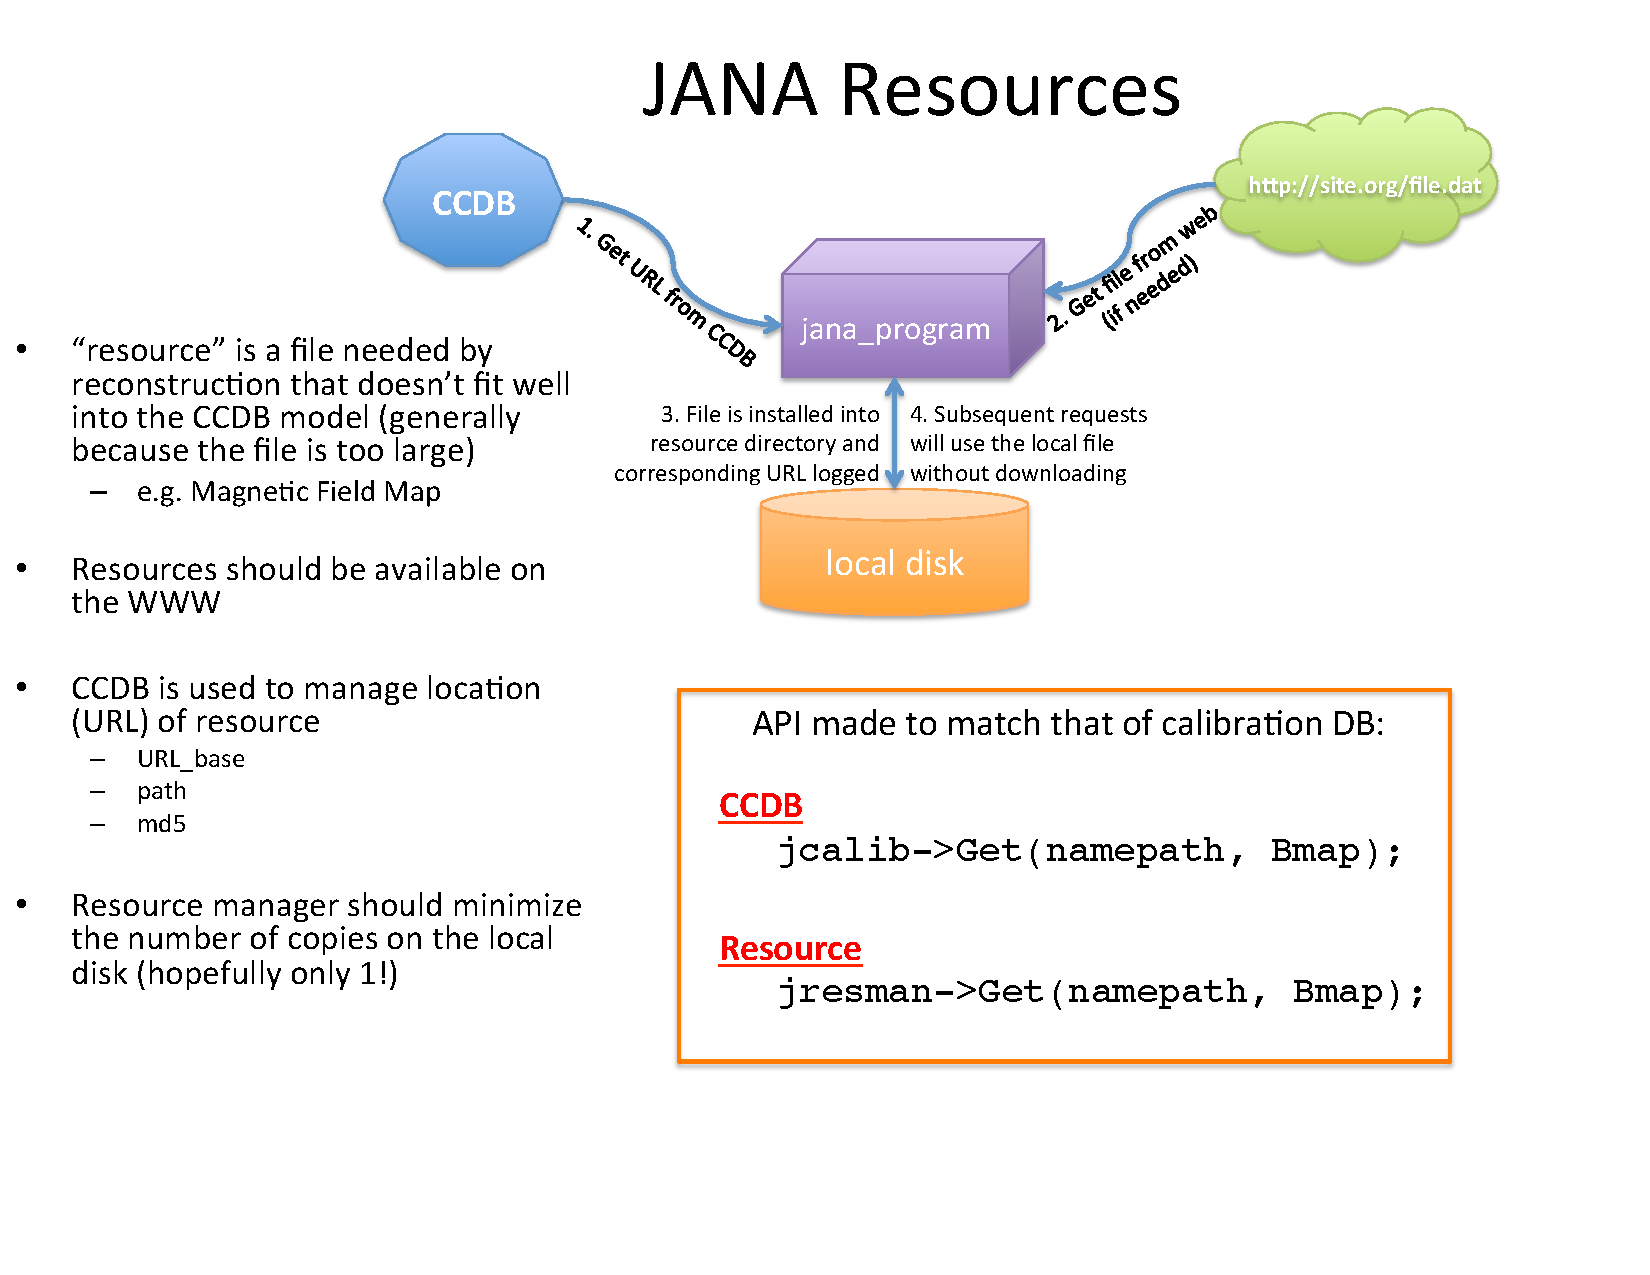
\includegraphics[width=\textwidth]{resources.pdf}$$}

\f{\ft{Geant4}
\bi
\I  progress on geometry
\I  Richard described changes needed last collab. meeting; G4 pickier than G3
\I  changes are done to both; required for apples-to-apples comparison
\I  some side-effects of those changes lingered and needed to be been addressed; done now
\ei
}

\f{$$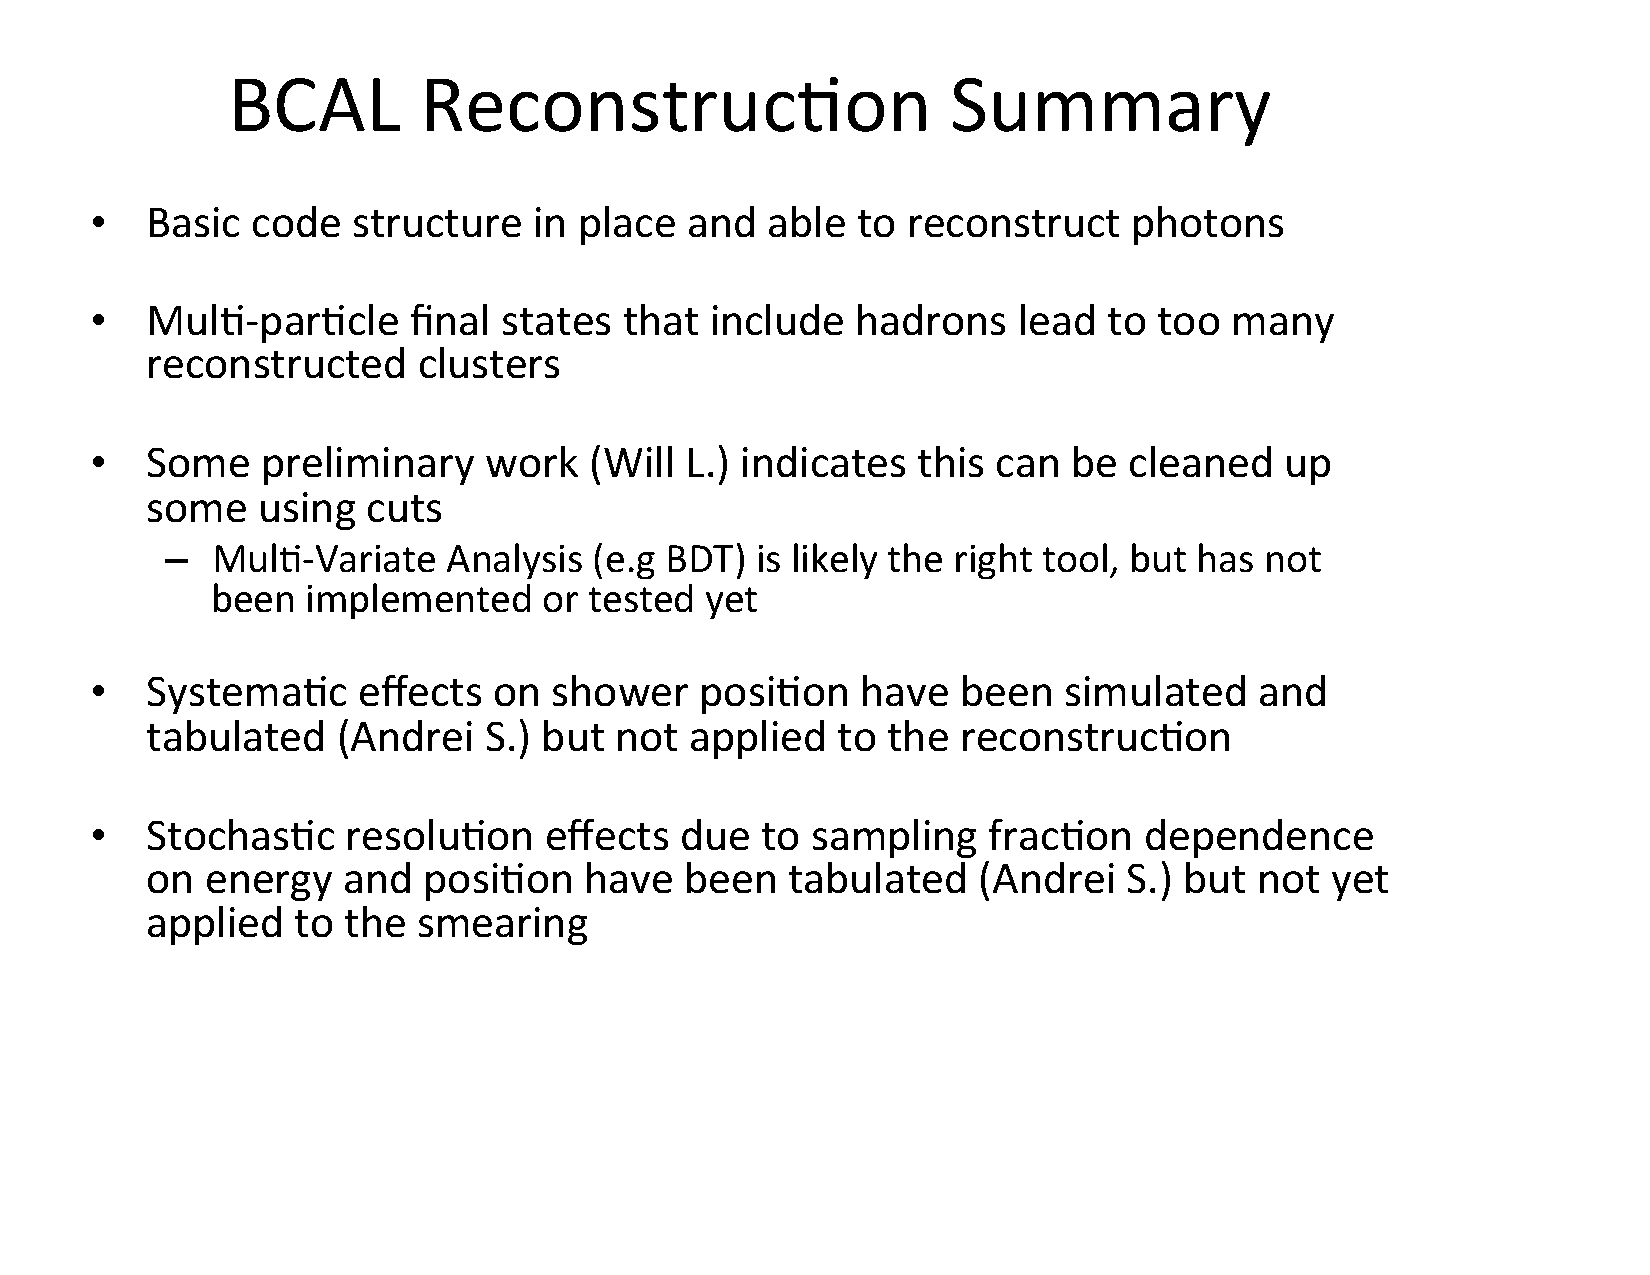
\includegraphics[width=\textwidth]{bcal_recon.pdf}$$}

\f{$$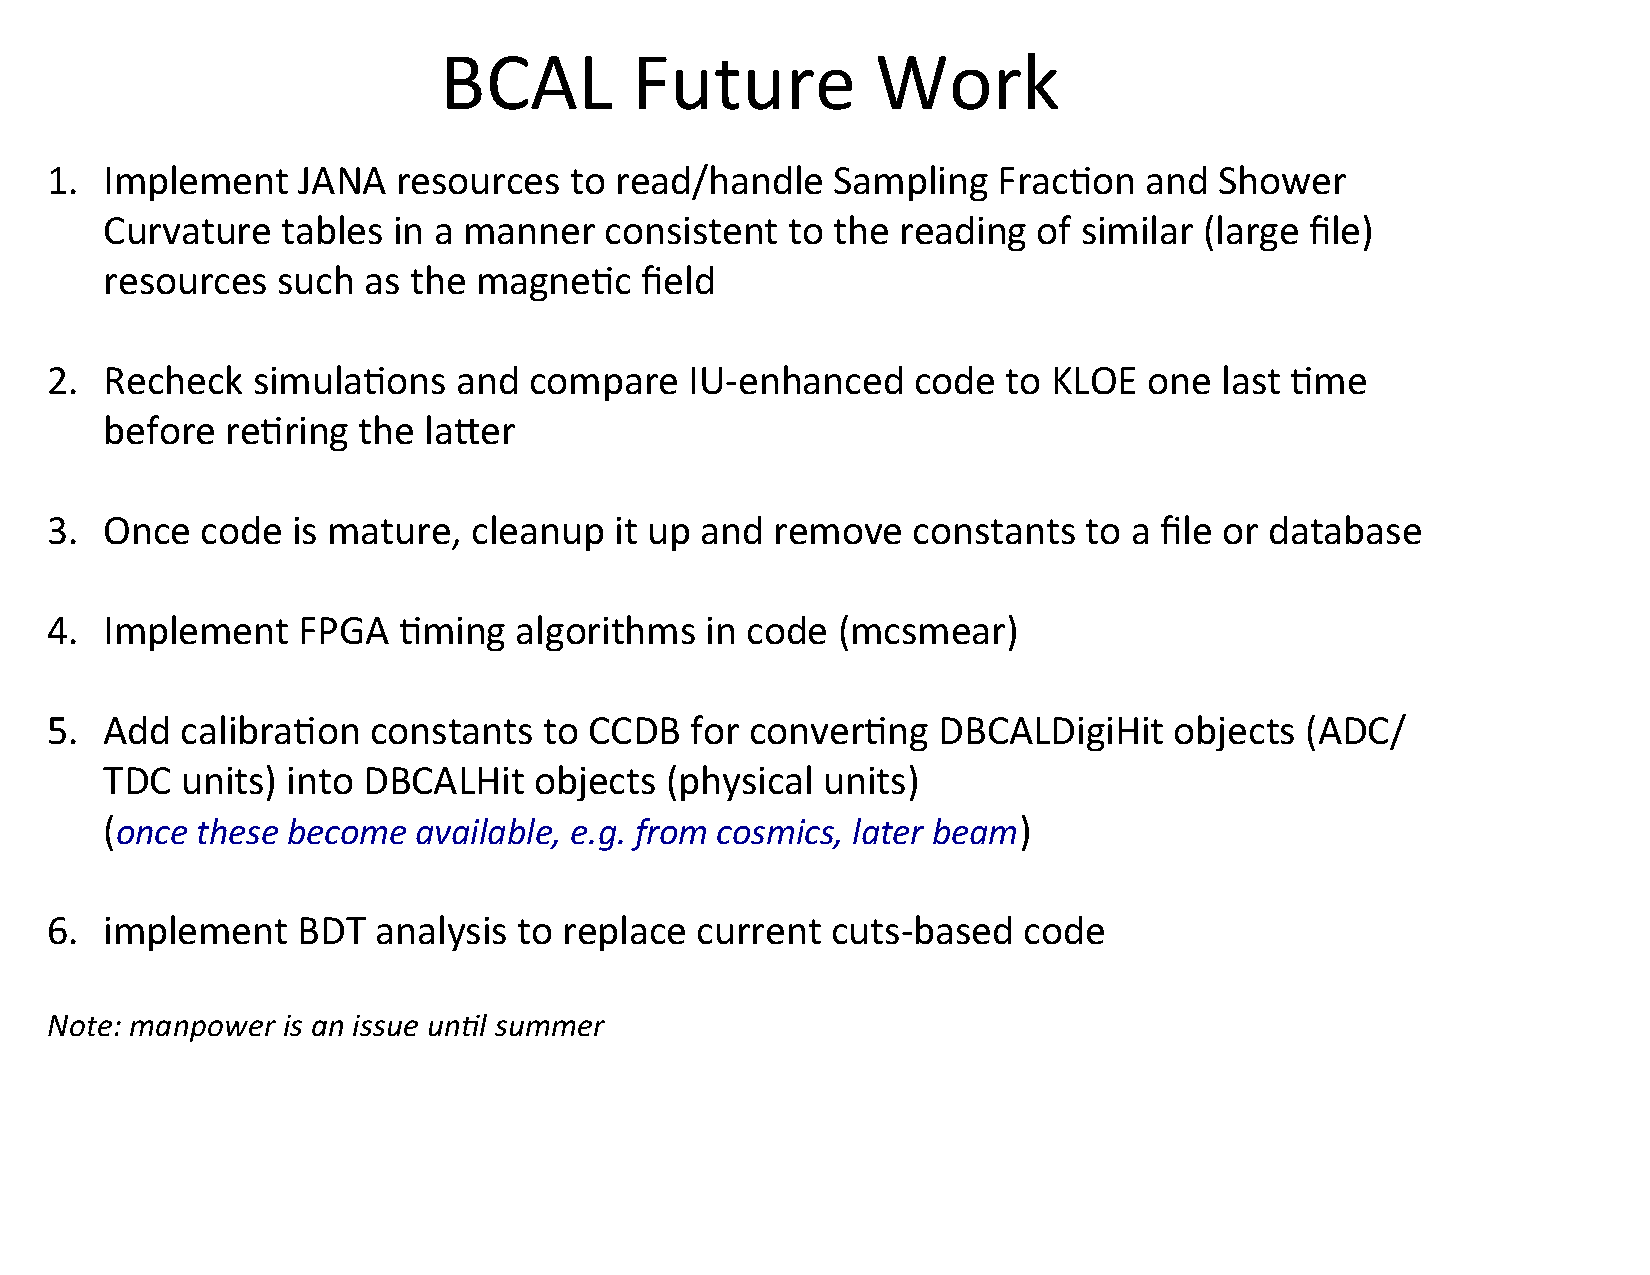
\includegraphics[width=\textwidth]{bcal_future.pdf}$$}

\end{document}
